\resourceheading{3}{PTR Evidence-to-Support Planning Guide}{Positive \& proactive behavior support}{Teachers, families \& support teams}{Module 2 Prevent--Teach--Reinforce assignment and a non-identifying placement event}

\vspace{-0.5cm}
\toolsection{What This Resource Is}

Prevent--Teach--Reinforce (PTR) is a team-based process for defining a concern observably, examining context and possible function, designing a linked plan, and reviewing both outcomes and implementation fidelity \citep{dunlap2019ptr}. This guide keeps observation, inference, hypothesis, and support decisions separate. Teams gather multiple observations, build a provisional hypothesis, and then link supports to what the evidence suggests. PTR supports communication and behavior when \textit{Prevent}, \textit{Teach}, and \textit{Reinforce} address the same access problem. Prevention changes conditions that make communication difficult. Teaching creates a safer or more efficient way to express the same need. Reinforcement makes that communication effective through a meaningful outcome rather than rewarding surface compliance.

\toolsection{Use This Guide Before Writing a Plan}
% \small
\renewcommand{\arraystretch}{1.0}
\setlength{\tabcolsep}{2.5pt}

\begin{longtable}{
>{\bfseries\RaggedRight\arraybackslash}p{0.70in}
>{\RaggedRight\arraybackslash}p{1.70in}
>{\RaggedRight\arraybackslash}p{2.00in}
>{\RaggedRight\arraybackslash}p{2.52in}}

\tableheaderfour{Step}{Record}{Ask}{Example Support}

Observe &
Actions, words, timing, task, tools, people, sensory conditions, and adult responses &
What can another observer verify? What remains unknown? &
``Adult reached for laptop; learner raised voice and held device.'' \\

\rowcolor{SoftGray}
Hypothesize &
A provisional relationship among conditions, communication, and outcome &
What other explanations fit? What student/family knowledge is missing? &
Familiar tool may support predictability, regulation, continued access, or something else. \\

Prevent &
Barrier changes before escalation &
Can the transition be previewed, modeled, overlapped, or chosen? &
Visible warning; laptop beside blocks; observe-first or partner-start option. \\

\rowcolor{SoftGray}
Teach &
A message or participation route that serves the same purpose &
Can the learner say it through speech, writing, gesture, AAC, or pointing? &
\textit{Not yet, more time, keep this with me, show me, help, break.} \\

Reinforce &
Natural response that makes the new route reliable &
Does the message change what happens when safety allows? &
More time occurs; familiar tool remains; learner enters through a chosen route. \\

\rowcolor{SoftGray}
Review &
Student outcomes and adult implementation &
Was the option available, recognized, honored, and useful? &
Track communication, participation, distress, trust, access, and fidelity. \\
\end{longtable}

\normalsize
\begin{center}

\begin{minipage}[c]{0.70\textwidth}
\centering
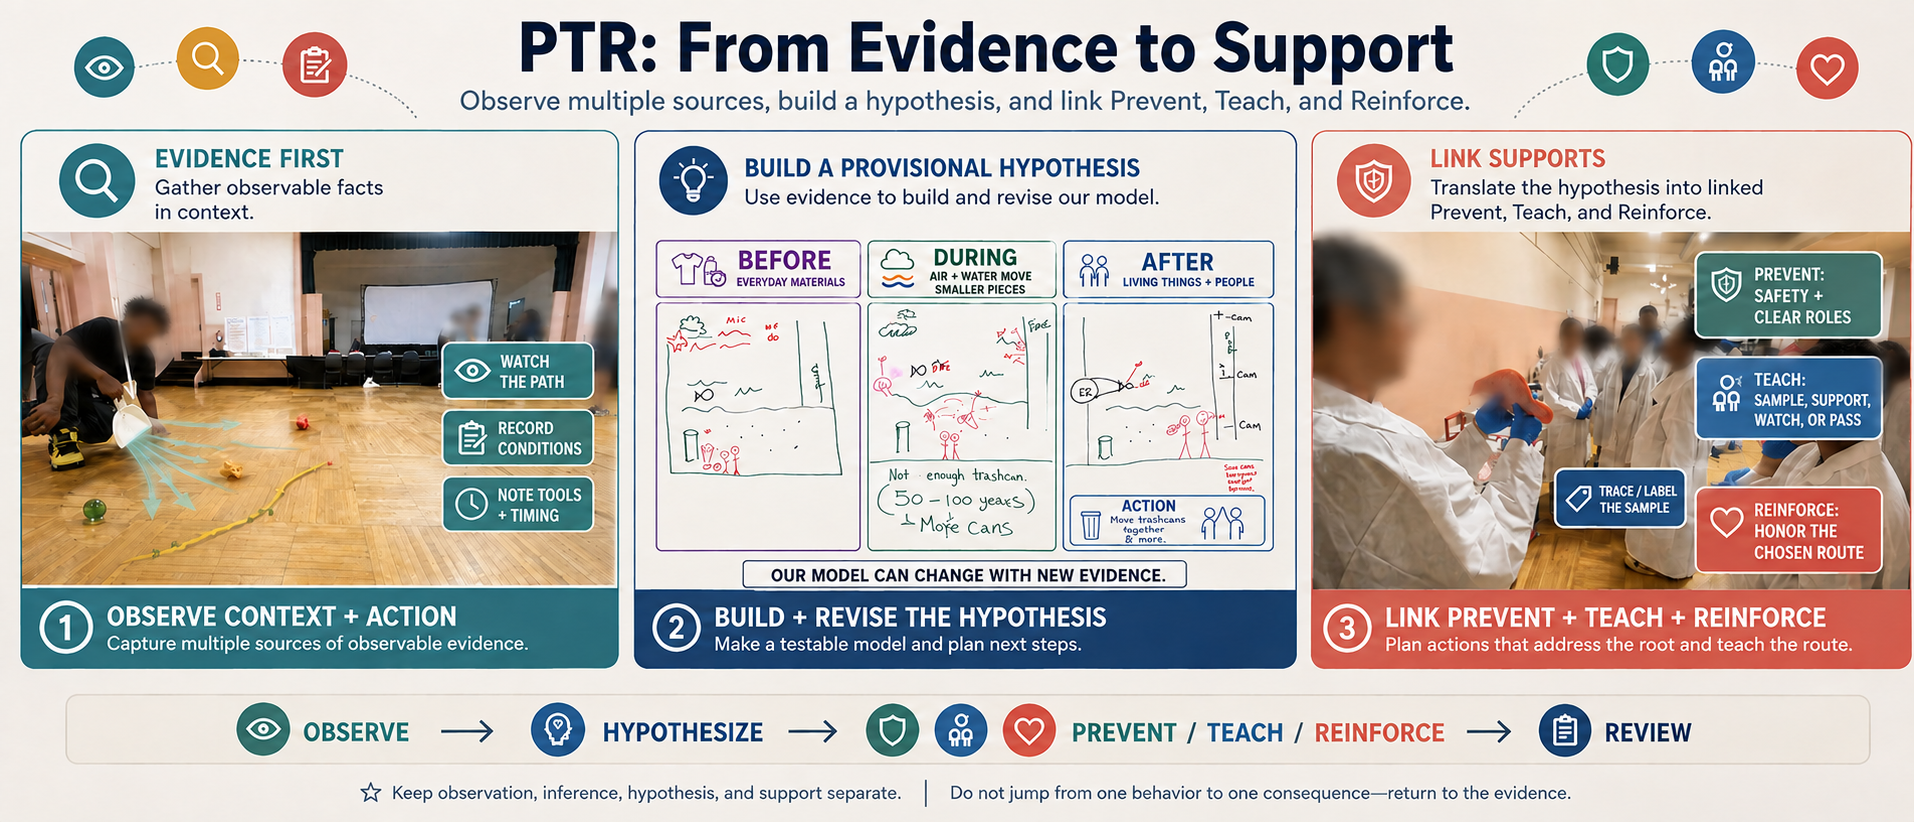
\includegraphics[
  width=0.90\linewidth,
  keepaspectratio
]{assets/artifact-previews/from_evidence_to_support.png}
\end{minipage}
\hfill
\begin{minipage}[c]{0.29\textwidth}
% \scriptsize
\RaggedRight
{\centering\bfseries\color{DeepNavy} From Evidence to Support.\par}
{\centering Camp practice illustrates the same planning logic: observable conditions and actions provide evidence, multiple pieces inform a provisional model, and that model guides linked supports. New evidence then returns the team to review and revision.\par}
\end{minipage}

\end{center}

\newpage
\toolsection{Completed Assignment Artifact: Appendix 4.1 Snapshot}

A public companion to the official checklist made uncertainty visible instead of filling gaps with assumptions:

\small
\renewcommand{\arraystretch}{1.13}
\setlength{\tabcolsep}{5pt}

\begin{tabularx}{\textwidth}{
>{\bfseries\RaggedRight\arraybackslash}p{1.36in}
>{\RaggedRight\arraybackslash}X}

\rowcolor{PrimaryRed}
\color{white}Checklist Area &
\color{white}Evidence-Supported Entry \\

Most associated routine &
Transition from familiar laptop use to a hands-on blocks activity; attempted device removal immediately preceded protest. \\

\rowcolor{SoftGray}
Least associated routine &
Unknown. Increased participation after the laptop remained is a response-to-support observation, not a stable pattern. \\

Provisional hypothesis &
Abrupt removal may have made the transition harder; preserving laptop access may have supported predictability, regulation, continuity, communication, preferred activity, or another function. \\

\rowcolor{SoftGray}
Evidence still needed &
Learner and family perspective; repeated observations; current IEP supports; latency, communication route, adult fidelity, and participation across conditions. \\

\end{tabularx}

\normalsize

Implementation commitments are to build the team with the learner and family, collect repeated baseline evidence, link all three PTR components to one hypothesis, include adult and environmental actions, and decide what evidence will trigger a keep/change/stop decision.

\begin{center}
\begin{minipage}[c]{0.62\textwidth}
\centering
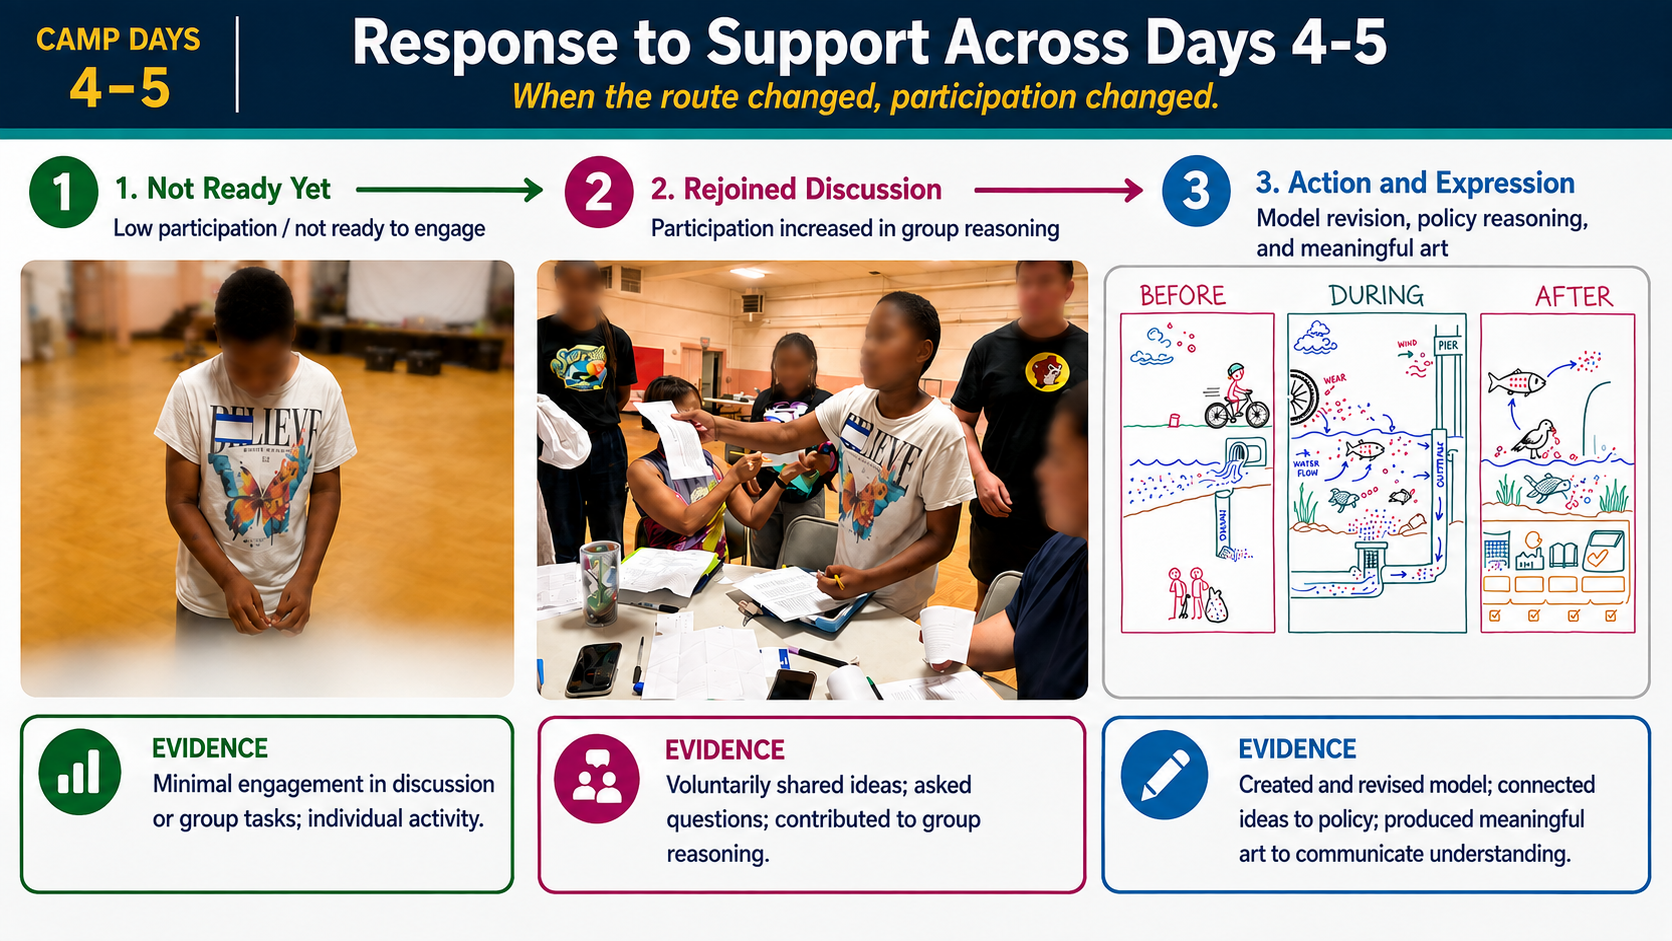
\includegraphics[
  width=\linewidth,
  keepaspectratio
]{assets/artifact-previews/response_to_support_across_days_4_5.png}
\end{minipage}
\hfill
\begin{minipage}[c]{0.37\textwidth}
% \scriptsize

{\centering\bfseries\color{DeepNavy} Evidence Boundary.\par}

{\centering The camp sequence documents increased participation after support changed: from not being ready to engage, to group reasoning, and then to action and expression. It shows a response to support over time, not a confirmed behavioral function.\par}

\end{minipage}
\end{center}

Constructing communicative competence requires more than presuming it: educators must make useful communication available and consequential throughout the day \citep{jorgensen2018competence}. A learner should not have to surrender a familiar support, become quiet, make eye contact, or follow an adult's preferred schedule to demonstrate success. Gardner's first-hand report warns that apparently effective intervention can still produce masking, shame, or weaker boundaries when conformity is the real outcome \citep{gardner2017firsthand}.

\reflectionbox{The Module 2 case began with one documented transition: an adult attempted to remove a familiar laptop before a blocks activity; after the either--or condition was removed, the learner joined the building activity while keeping the laptop nearby. This does not establish a behavioral function or a universal laptop intervention. Like the camp sequence above, it shows why changes in conditions and participation belong in the evidence record. Puzzle Plan keeps those conditions visible; EQUITAS keeps the learner and family able to contest the team's interpretation. ``Unknown'' is an accountable finding when the data do not support a conclusion.}

\adaptationbox{PTR can be misused when teams select compliance goals, ignore communication modes, or count only student behavior. Review cultural and family meaning, sensory and health conditions, language access, and whether the learner can disagree with the team's interpretation. If visible behavior decreases while communication, trust, participation, or quality of life also decreases, the plan is not positive and should be revised.}

\sourcebox{PTR second edition \citep{dunlap2019ptr}; communication competence \citep{jorgensen2018competence}; first-hand intervention perspectives \citep{gardner2017firsthand}.}